%\documentclass[11pt,professionalfonts,hyperref={pdftex,pdfpagemode=none,pdfstartview=FitH}]{beamer}
%\usepackage{times}
\documentclass[11pt,professionalfonts]{beamer}
\usefonttheme{serif}
\usepackage{presentation_packages}
\usepackage[version=3]{mhchem}
\DeclareSIUnit\year{yr}
\newcommand{\hilight}[1]{\colorbox{green}{#1}}

\definecolor{mygray}{gray}{0.9}
\definecolor{RoyalBlue}{rgb}{0.25,0.41,0.88}
\def\Emph{\textcolor{RoyalBlue}}

\definecolor{tmp}{rgb}{0.804,0.941,1.0}
\setbeamercolor{numerical}{fg=black,bg=tmp}
\setbeamercolor{exact}{fg=black,bg=red}

\mode<presentation> 
{
  \usetheme{Warsaw}
  \usefonttheme{serif}
  \setbeamercovered{transparent}
}

\setbeamertemplate{footline}%{split theme}
{%
  \leavevmode%
  \hbox{\begin{beamercolorbox}[wd=.5\paperwidth,ht=2.5ex,dp=1.125ex,leftskip=.3cm,rightskip=.3cm plus1fill]{author in head/foot}%
    \usebeamerfont{author in head/foot}\insertshorttitle
  \end{beamercolorbox}%
  \begin{beamercolorbox}[wd=.5\paperwidth,ht=2.5ex,dp=1.125ex,leftskip=.3cm,rightskip=.3cm]{title in head/foot}
%    \usebeamerfont{title in head/foot}\mypaper\hfill \insertframenumber/\inserttotalframenumber
    \usebeamerfont{title in head/foot}\hfill \insertframenumber/\inserttotalframenumber
  \end{beamercolorbox}}%
  \vskip0pt%
} \setbeamercolor{box}{fg=black,bg=yellow}


\title[Asteroid Reconstruction]{\large\textbf Real Time asteroid reconstruction}

\author{\vspace*{-0.3cm}}
   
\institute{
	\footnotesize
	{\normalsize\bf{Shankar Kulumani, Kuya Takami \\ Taeyoung Lee}}\\
	\vspace*{0.2cm}
  	\textbf{Department of Mechanical \& Aerospace Engineering}\\ \vspace*{0.5cm}
 	\begin{figure} %figure%
       	
\includegraphics[width=0.75\textwidth]{gw_txh_2cs_pos}
  	\end{figure}
}
\date{August 23, 2017}

\begin{document}
%=======================================================%

\setcounter{framenumber}{-1}
\begin{frame} %-----------------------------%
  \titlepage
\end{frame}   %-----------------------------%

\section*{}
\subsection*{Introduction}  
\begin{frame}{Asteroid Missions}
\begin{itemize}
    \item Science - insight into the early formation of the solar system
    \item Mining - vast quantities of useful materials
    \item Impact - high risk from hazardous near-Earth asteroids
\end{itemize}    

\begin{center}
    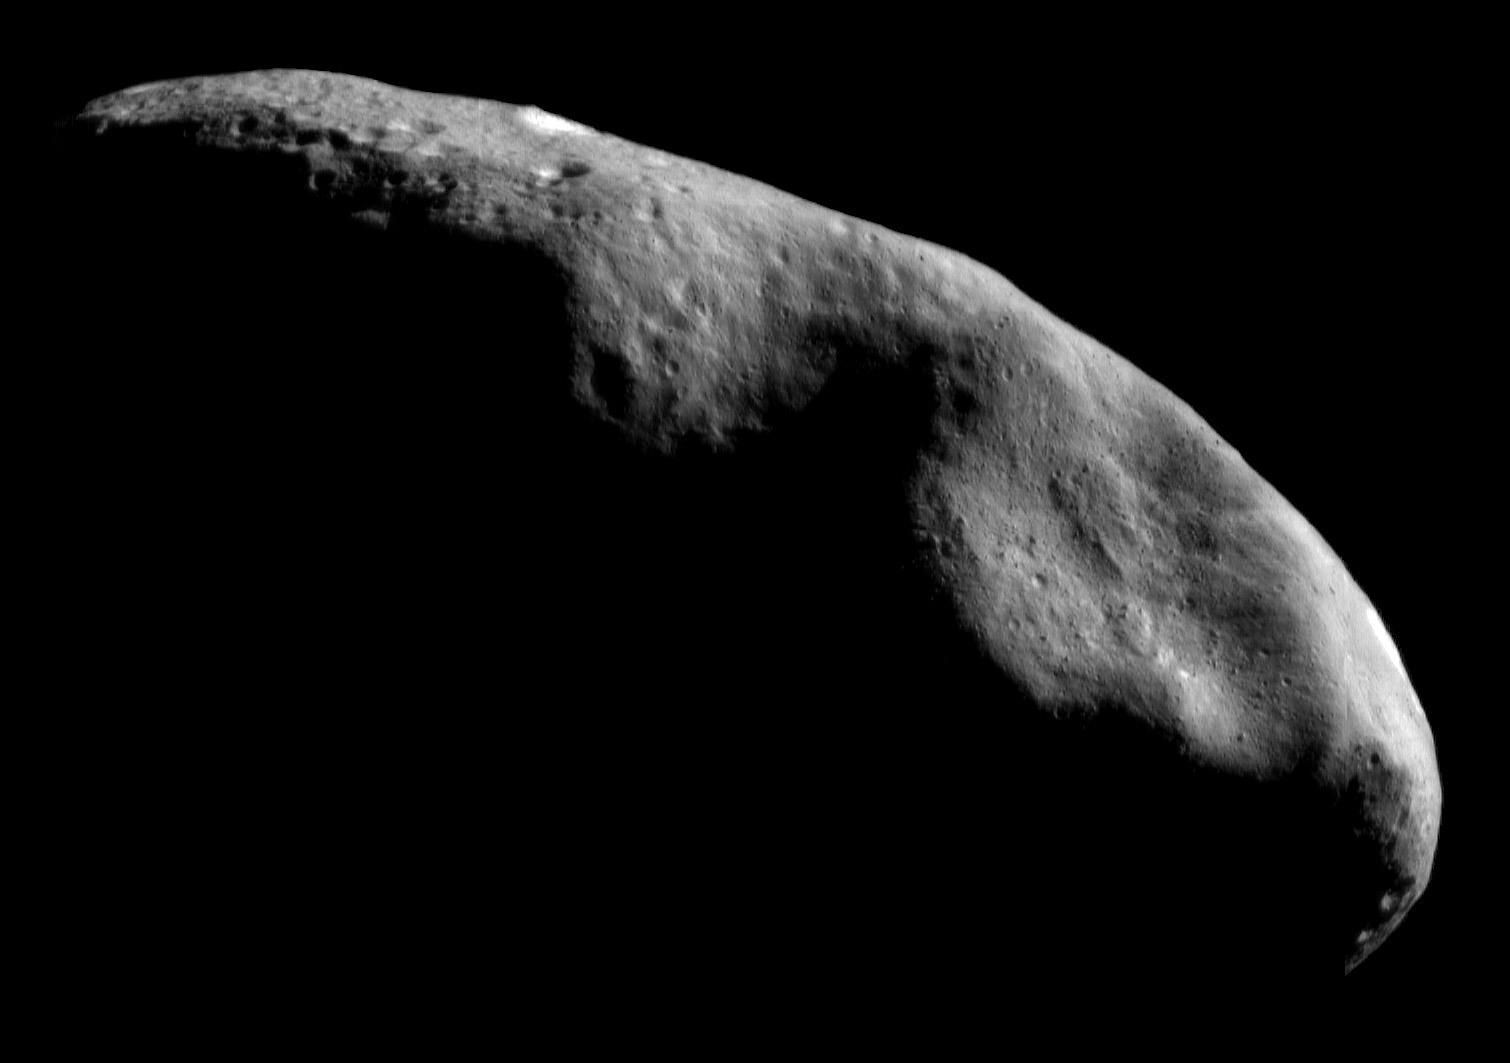
\includegraphics[height=0.35\textheight]{figures/near_mos_20001203_full.jpg}
    \hfill
    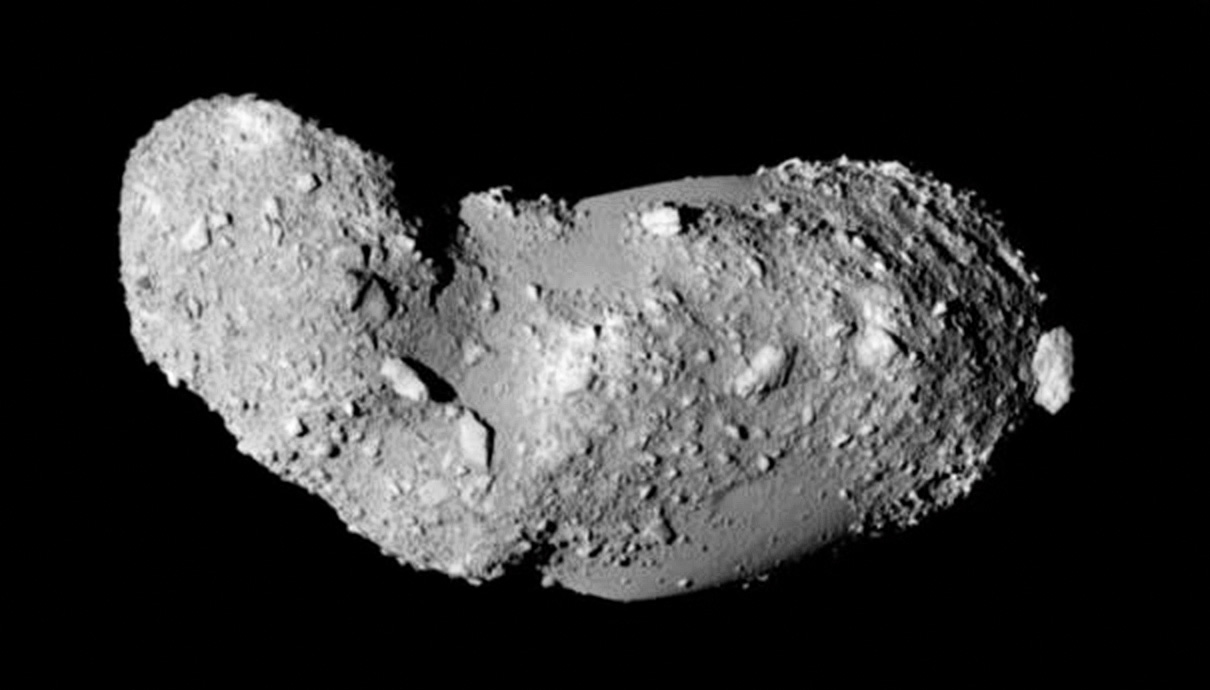
\includegraphics[height=0.35\textheight]{figures/Itokawa8_hayabusa_1210.jpg}
\end{center}
\end{frame}

\begin{frame}{Asteroid Mining}
    \begin{itemize}
      \item Useful materials can be extracted from asteroids to support:
      \begin{itemize}
          \item Propulsion, construction, life support, agriculture, and precious/strategic metals
      \end{itemize}
        \pause
      \item Commercialization of near-Earth asteroids is feasible
    \end{itemize}


\begin{center}
\small
    \begin{tabular}{|l|r|r|}
        \hline 
        Element & Price (\SI{}[\$\,]{\per\kilo\gram}) & Sales (\SI{}[\$\,]{M\per\year}) \\
        \hline \hline 
        Phosphorous (P) & \num{0.08}  & \num{2167} \\
        Gallium (Ga) & \num{300.00}  & \num{1544} \\
        Germanium (Ge) & \num{745.00} & \num{6145} \\
        \hline \hline 
        Platinum (Pt) & \num{12394.00} & \num{1705} \\
        Gold (Au) & \num{12346.00} & \num{49} \\
        Osmium (Os) & \num{12860.00} & \num{307} \\
        \hline
    \end{tabular}
\end{center}

\end{frame}

\section*{}
\subsection*{Motivation}  
\begin{frame}{Asteroid Landing}
    \begin{itemize}
        \item Long history of asteroid/planetary missions
            \begin{itemize}
                \item NEAR, Hayabusa, OSIRIS-REX, Rosetta
            \end{itemize}
            \pause
        \item Asteroid landing is particularly challenging:
            \begin{itemize}
                \item<3-> Challenging dynamics - unknown gravity enviornment
                \item<4-> Poor shape model - unknown surface topography from the ground
                \item<5-> Attitude coupling - pertubations are large 
            \end{itemize}
    \end{itemize}
    \begin{center}
        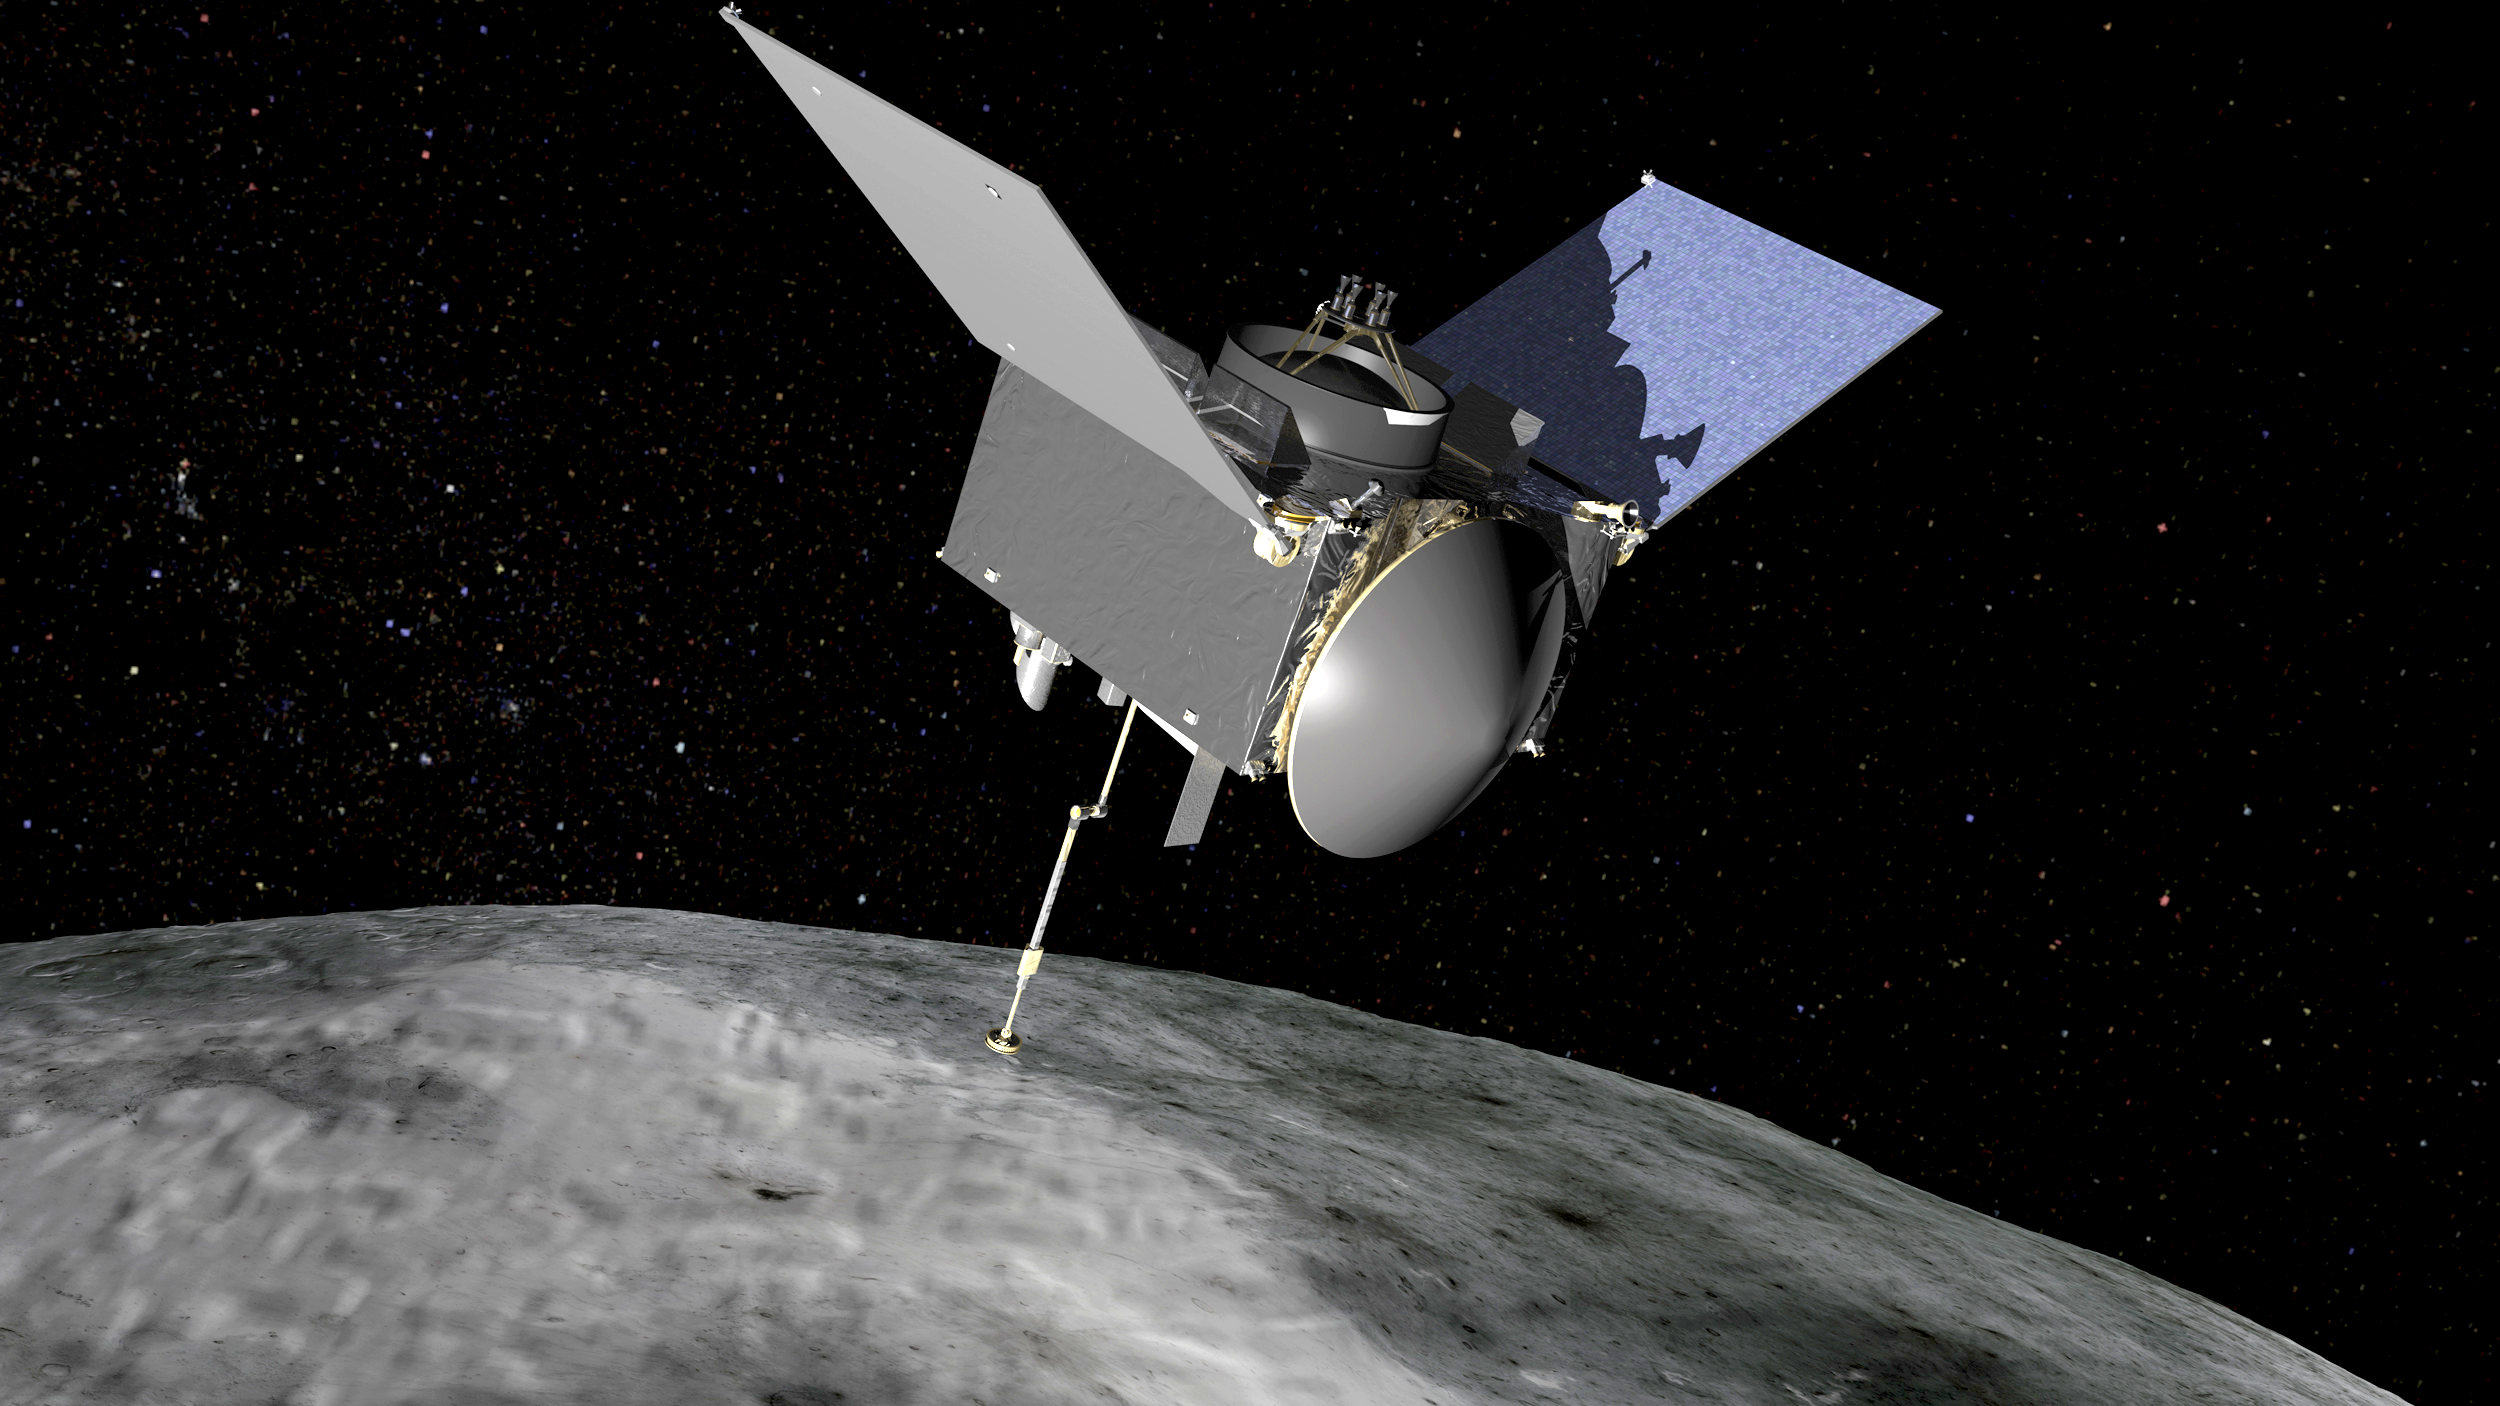
\includegraphics[width=0.6\textwidth,height=0.4\textheight,keepaspectratio]{figures/osiris_rex.png}~
        \includegraphics[width=0.6\textwidth,height=0.4\textheight,keepaspectratio]{figures/Rosetta_Philae_Artist_Impression_Close_4k.jpg}
    \end{center} 
\end{frame}

\begin{frame}{Challenges in Asteroid Missions}
    \begin{itemize}
        \item Very challenging dynamic enviornment
            \begin{itemize}
                \item Highly irregular shape and chaotic spin states
                \item Difficult to identitfy and track from the ground
                \item Poor understanding upon spacecraft arrival
            \end{itemize}
        \item Coupled translational and rotational dynamics
            \begin{itemize}
                \item Spacecraft is relatively large compared to the orbit radius
                \item Complex interaction between the attitude and position forces
                \item Magnified at lower altitudes and with highly irregular shapes
            \end{itemize}
        \item Critical to accurately model the gravitational force
            \begin{itemize}
                \item 
            \end{itemize}
    \end{itemize}
\end{frame}

\begin{frame}{Problem Statement}
\begin{enumerate}
        \item Develop copuled equations of motion for a spacecraft
        \item EOMs on \( \SE \) to derive landing control law
            \begin{itemize}
                \item \( \SE \) - special euclidean group describes the general motion of rigid bodies
            \end{itemize}
        \item Implement monocular localization to provide state estimates
        \item Alleviates many of the issues of past approaches:
            \pause
            \begin{itemize}
                \item Explicitly consider rotational dynamics
                \item Geometric control defined directly on \( \SE \)
                \item Onboard state measurements for ``autonomy''
            \end{itemize}
    \end{enumerate}
\end{frame}

\section*{}
\subsection*{Conclusions}

\begin{frame}{Conclusions}
    \begin{itemize}
        \item Nonlinear controller for landing on an asteroid
        \item Coupled dynamics derived and considered on \SE
        \item Localization performed using simulated monocular imagery
        \item Future Research Goals:
            \begin{itemize}
                \item Utilize state estimates directly in controller
                \item Update shape and gravity model in real-time
            \end{itemize}
    \end{itemize} 
\end{frame}

\begin{frame}[c]{Thank you}
  \centering
  
  \textbf{\large Flight Dynamics \& Control Lab} \\
  Mechanical \& Aerospace Engineering \\
  School of Engineering \& Applied Science
  
  \begin{figure} %figure%
        
\includegraphics[width=0.75\textwidth]{gw_txh_2cs_pos}
    \end{figure}
  
  \url{https://fdcl.seas.gwu.edu}
\end{frame}
\end{document}

